%*************************************************************************************************************************
\section[The Thermal-Hydraulics System Code TRACE]{The Thermal-Hydraulics (TH) System Code TRACE}\label{sec:reflood_trace}
%*************************************************************************************************************************

% What is actually a system code
A \glsfirst[hyper=false]{th} system code is a computer code used to analyze the \gls[hyper=false]{th} behavior of \glspl[hyper=false]{npp} \cite{Roth2014}.
\marginpar{Thermal-hydraulics system code}
Its current usage ranges from safety analysis and licensing process of current reactor designs to qualification of a new reactor designs \cite{Petruzzi2008, Petruzzi2016}.
To that end, the code is designed to be a comprehensive tool capable of simulating wide range of operating conditions, 
from normal operations, anticipated transients, to accident scenarios foreseen in nuclear power plant operation.

% Component-based system code
A nuclear reactor system is a complex system of numerous interconnected components, each serving distinct purposes, built with multiple engineered safety features.
\marginpar{Nuclear reactor system}
During a transient, the system might exhibit complex behavior with physical phenomena interacting at vastly different time scales ($10^{-1} \, [s]$ in a power excursion due to control rod ejection, $10^5 \, [s]$ for decay heat removal after successful reactor shutdown) and
length scales ($10^{-3} \, [mm]$ for boiling at sub-channel level, $10^3 \, [m]$ for coolant flow in the primary/secondary circuit).
Additionally, the engineered safety features are designed for some equipments (such as control rods, valves, pump, etc.) to perform safety-related actions.
Such equipments, in turn, are controlled by a complex dynamical control system.
As such, system code has to take into account these different aspects to properly simulate the thermal-hydraulics behavior of nuclear power plants.
Indeed, com\-ponent-based codes, such as \gls[hyper=false]{trace}, approach the problem by representing each prominent component in a nuclear reactor system separately.
On top of a two-phase fluid dynamics equation solver, system code includes models for steam separator, pump, heat exchanger, valve, pressurizer, and neutron-kinetics 
as well as comprehensive models for control system to mimic the signal monitoring and component actuation systems in a \gls[hyper=false]{npp}.
System thermal-hydraulics thus distinguishes itself by considering explicitly the geometry, materials, boundary conditions, various interconnecting components, and control systems that constitute an \gls[hyper=false]{npp} \cite{DAuria2012}.

% The essence of the problem tackled in thermal-hydraulics system code
However, it can be argued that the modeling of two-phase flow inside a heated channel remains a central part in nuclear thermal-hydraulics analysis 
\marginpar{basic thermal-hydraulics, two-phase flow in a heated channel}
which puts an emphasis in the correct prediction of cladding temperature evolution during different postulated scenarios (Fig.~\ref{fig:ch2_heated_channel}). 
This is also supported by the fact that the majority of operating nuclear power plants is of \gls[hyper=false]{lwr} type, 
where two-phase flow can be expected to occur during its operation, both in normal operating and accident conditions for \glspl[hyper=false]{bwr} and in accident condition for \glspl[hyper=false]{pwr}.
\begin{figure}[bth]
	\centering
	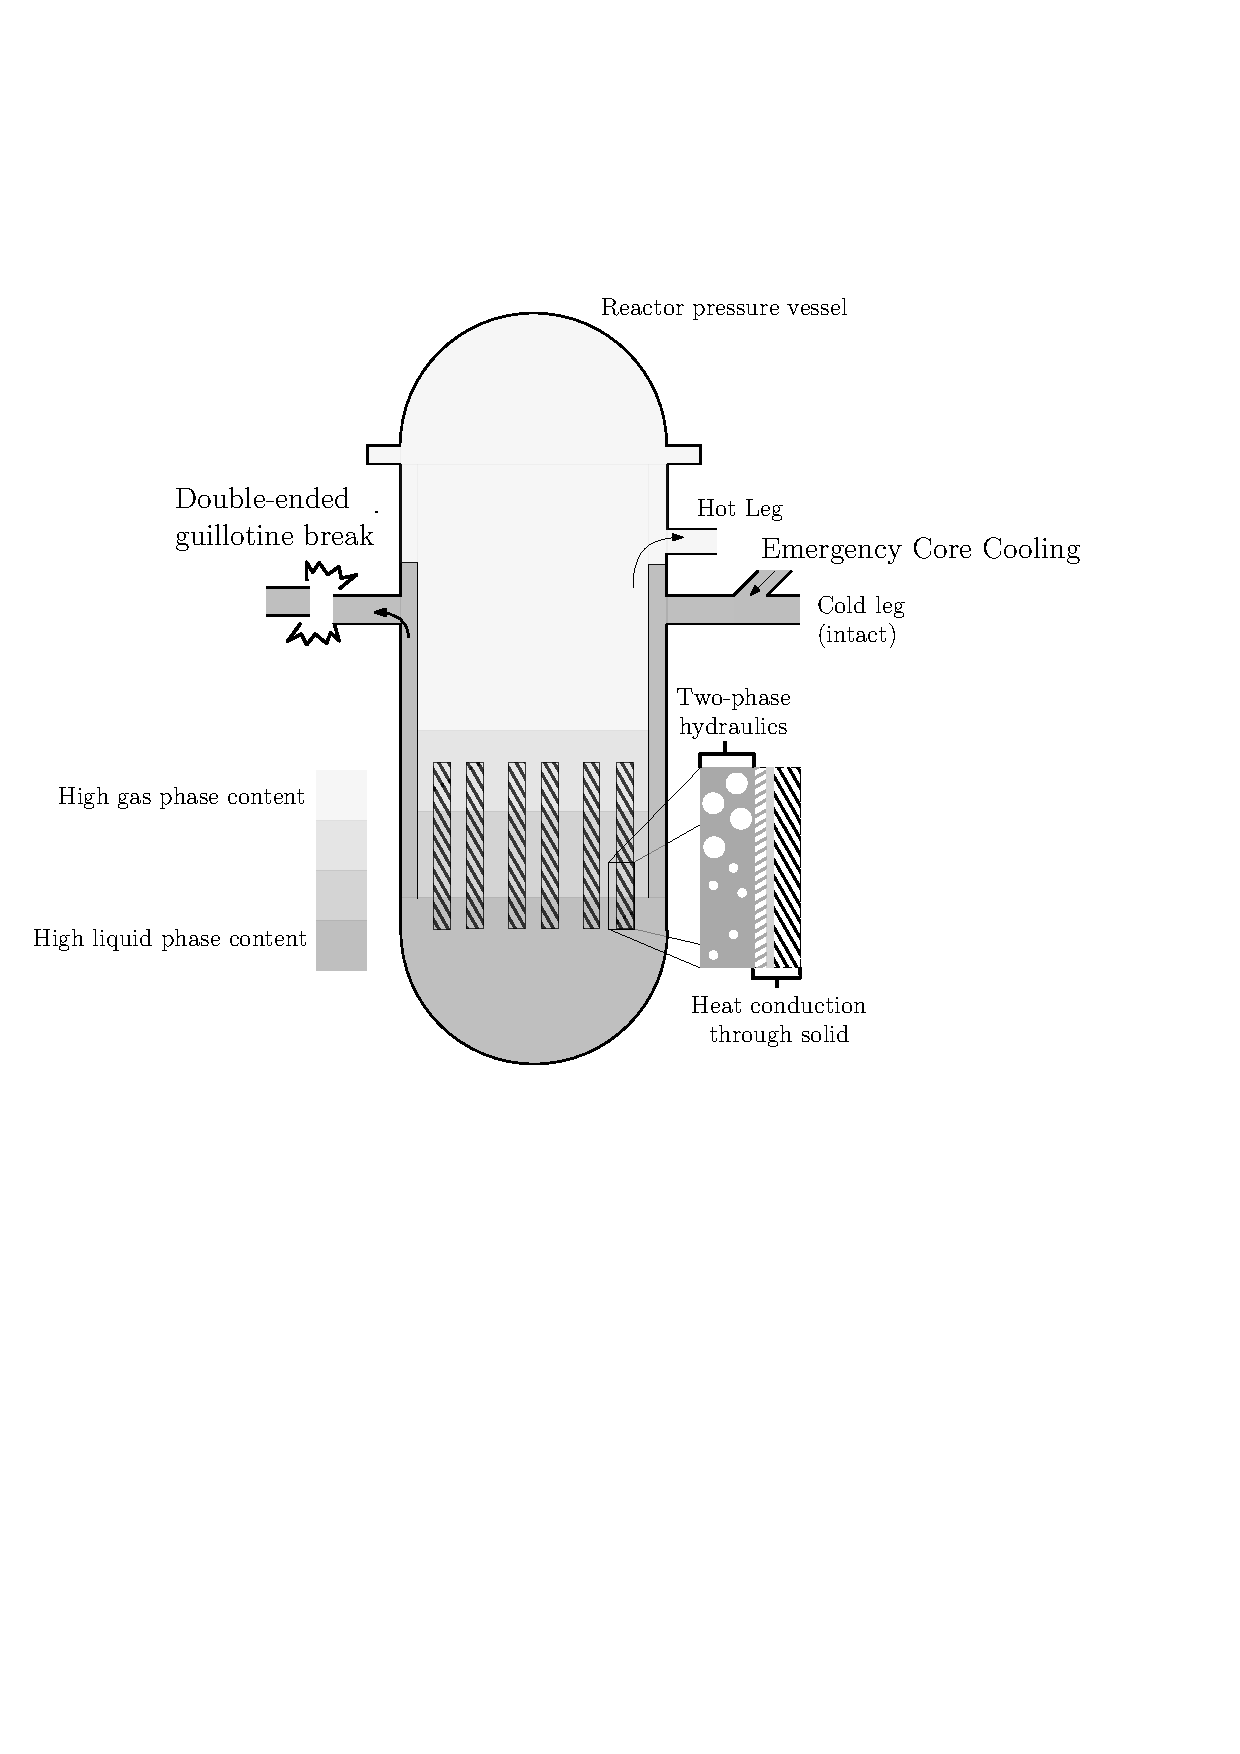
\includegraphics[scale=0.55]{../figures/chapter2/figures/heatedChannel}
	\caption[Illustration of Heated Channel.]{Thermal-hydraulics system analysis encompasses many aspects of nuclear reactor system analysis, but the core of the problem for predicting the cladding temperature evolution (especially during an accident condition) is to model properly and realistically the coolant flow in a heated channel in steady or transient conditions. Here it is shown a simplified picture of a \gls[hyper=false]{loca} in a \glsentryshort{pwr} where phase change occurs along the heated channel.}
	\label{fig:ch2_heated_channel}
\end{figure}

% Major difficulty
The problem of modeling properly the two-phase flow in a heated channel, though much more limited in scope, is by no means trivial.
\marginpar{flow regimes}
This is due to the fact that in two-phase flow, the morphological configurations of the flow (i.e., \emph{flow regimes}) can vary widely depending on many parameters such as differences in the respective phase density and velocity, as well as in the flow orientation.
Different flow regimes implies different interfacial surface structure between the two phases (see Fig.~\ref{fig:ch2_flow_regimes}), which in turn affects the mass, momentum, and energy coupling terms (\emph{transfer relation}) between the phases.
At the same time, the interfacial surface and its deformation in an arbitrary flow configuration are not known \emph{a priori} and becomes part of the problem to be simultaneously solved.
\begin{figure}[bth!]
	\centering
	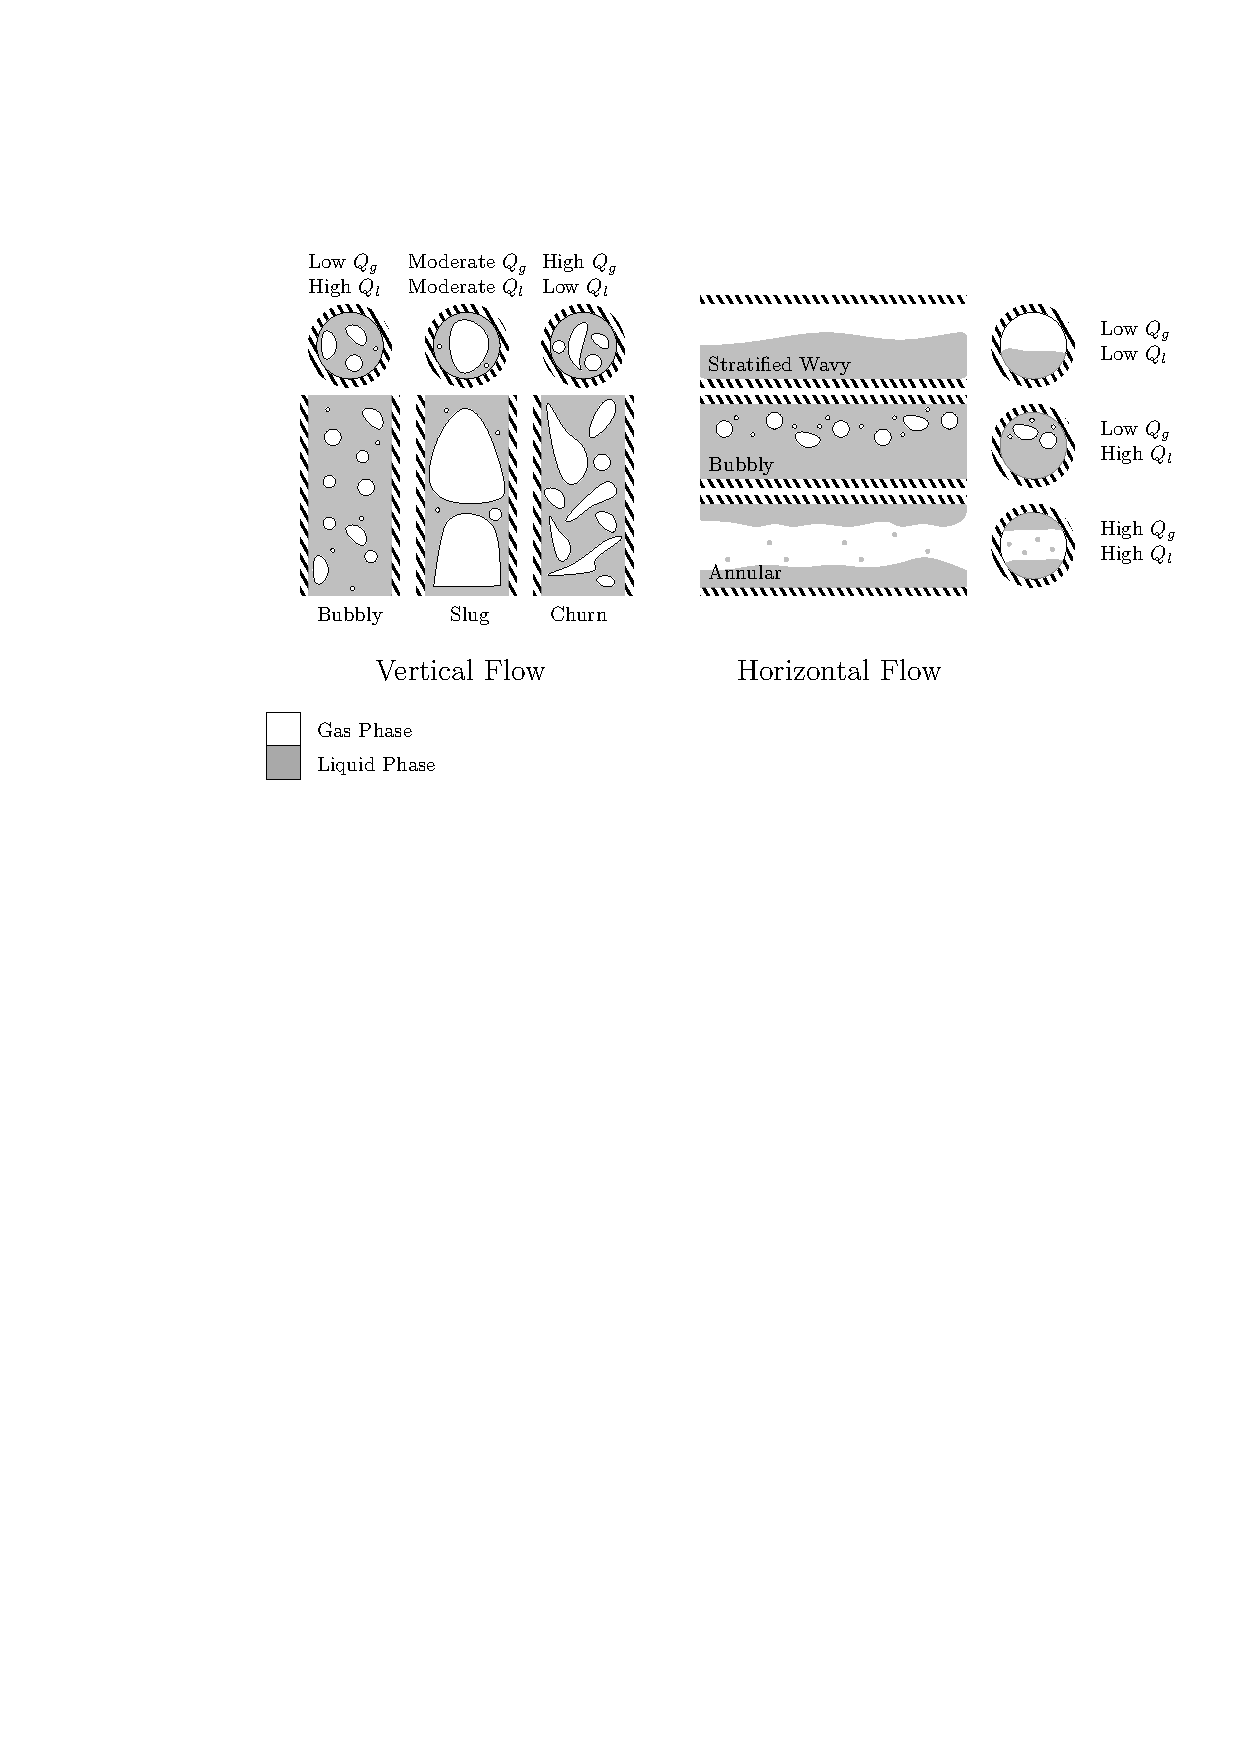
\includegraphics[width=\textwidth]{../figures/chapter2/figures/flowRegimes}
	\caption[Some of the observed flow regimes in vertical and horizontal flow]{Some of the observed flow regimes in vertical and horizontal flow with different superficial liquid velocity, $Q_l = V_l / A$, and superficial gas velocity, $Q_g = V_g / A$, where $A$ is the flow area. The flows of both phases are co-current.}
	\label{fig:ch2_flow_regimes}
\end{figure}

% The rigorous approach, local instantaneous formulation
The most rigorous approach in describing two-phase flow is by using local instantaneous formulation where a set of partial differential equations describing the conservation of mass, momentum, and energy, is formulated for each phase.
\marginpar{local instantaneous formulation, topological constraint}
The two phases are, in turn, separated by zero-thickness interfacial surfaces.
The resulting set of equations fully describes the flow at any given location and at any given time.
In addition, the solution of this formulation also respects the \emph{topological constraint} of the flow.
The constraint states that only one phase can exist at any given time and location in the flow \cite{Ghiaasiaan2007}.
This is illustrated in the Fig.~\ref{fig:ch2_phase_indicator_probe} where a hypothetical probe is put within a two-phase flow and a signal of indicator function $M(\mathbf{r}, t)$ is recorded.
\begin{figure}[bth!]
	\centering
	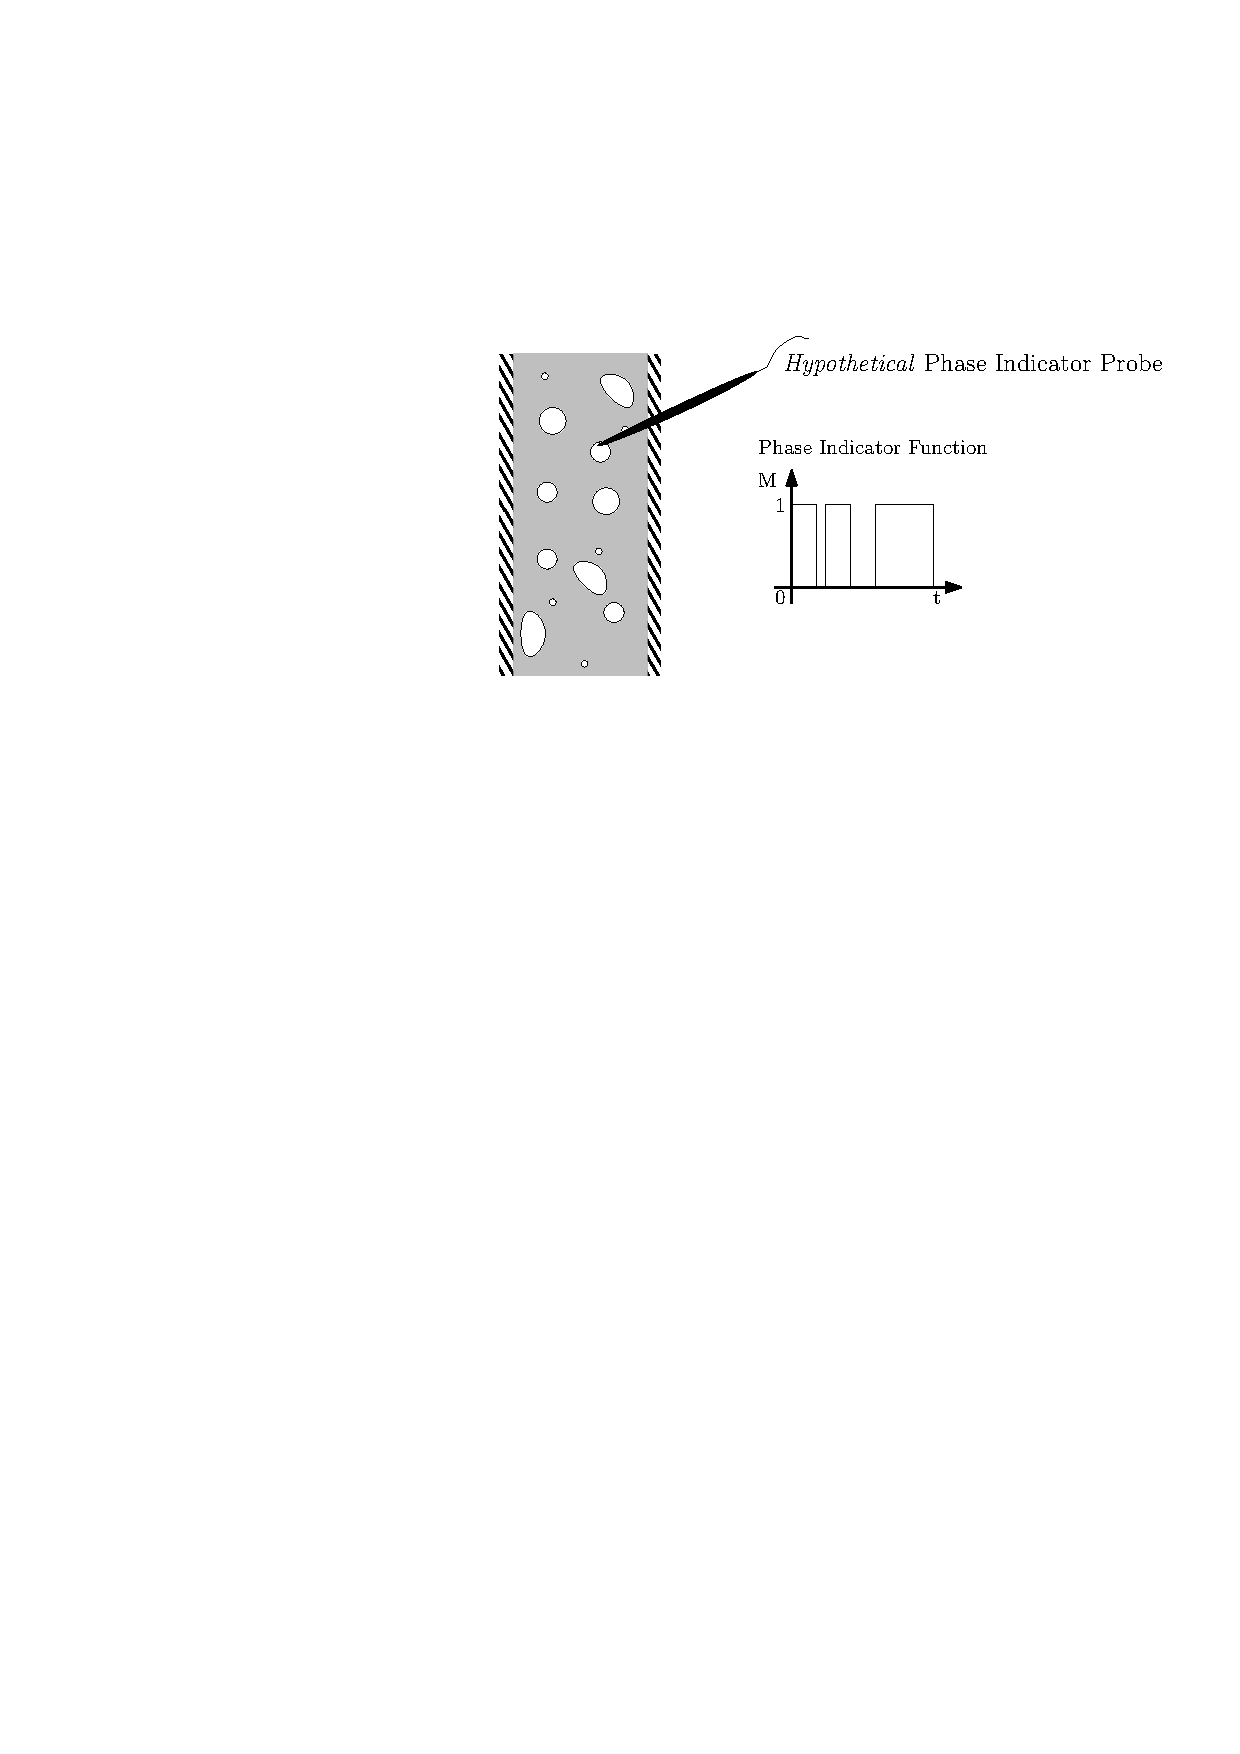
\includegraphics[scale=0.70]{../figures/chapter2/figures/phaseIndicatorProbe}
	\caption[A hypothetical phase indicator probe inside a channel of a two-phase flow]{Illustration of a hypothetical phase indicator probe inside a channel of a two-phase flow, recording the evolution of the indicator function (Eq.~(\ref{eq:indicator_function})) at a given point.}
	\label{fig:ch2_phase_indicator_probe}
\end{figure}

The indicator function $M(\mathbf{r}, t)$ is defined as,
\begin{equation}
  M (\mathbf{r}, t) =
    \begin{cases}
      1 \, ; \, \text{if probe tip is in the \text{gas phase}} \\
      0 \, ; \, \text{otherwise}
    \end{cases}
\label{eq:indicator_function}
\end{equation}
where \gls[hyper=false]{r} is position;
and \gls[hyper=false]{t} is the time.
The indicator function defined here is equivalent to the local instantaneous void fraction, 
which can be interpreted as the probability that the gas phase is present at a given point in space at a given moment \cite{USNRC2012}. 

As mentioned, the interfacial surface structure of the flow determines the coupling terms between the two phases.
\marginpar{resolving the motion of interfacial surface}
However, this surface and its deformation along the flow are not known \emph{a priori}.
As such, the solution of the local instantaneous formulation of two-phase flow requires to solve the motion of interfacial surface. 
As the time and length scales of the interfacial structure in a two-phase flow of an arbitrary morphological configuration can vary wildly,
the problem of resolving the motion of interfacial surface becomes intractable. 
Though advances have been made in the area of Computational Fluid Dynamics (CFD) in this regard, 
the problem remains intractable for the purpose of thermal-hydraulics system analysis\footnote{See \cite{Bestion2014} for a recent review on the topic.}.

% The simplified approach, Time and Volume Averaged
To simplify the intractability problem of resolving the motion of interfacial surface motion in two-phase flow inside a channel, time- and area-average is carried out on the flow.
\marginpar{Time- and volume (area)-averaging}
Averaging can be seen as a filtering operation to remove the local temporal and spatial fluctuations (short scale variation) in the flow.
The length and duration which define short scale variation are problem specific 
(that is, at least qualitatively, not longer than the length and time scales of the flow configuration of interest).
The volume over which averaging is carried out is referred to either as a \emph{control volume}, a \emph{cell}, or a \emph{node}.
It is further assumed that the flow is one-dimensional, in which the flow area changes slowly along the principal direction of the flow.
Under these assumptions, a control volume simply corresponds to a cross-sectional slice of the channel and the averaging is based on the flow area instead \cite{Ghiaasiaan2007}.

Averaging the indicator function both in time and in (a sliced) area gives the \emph{void fraction},
\begin{equation}
  \langle \bar{\alpha} \rangle =  \frac{1}{A\,\Delta t} \int_{A} \int_{t}^{t + \Delta t} M(\mathbf{r}, t)\,d\mathbf{r}\,dt
\label{eq:void_fraction}
\end{equation}
Following the above formulation, void fraction can be interpreted as the fraction of the control volume occupied by the gas phase \cite{USNRC2012}.

% Two fluid model and its closure
Averaging the flow state variables in time and area and using them to formulate a set of mass, momentum, and energy balance equations describing the fluid dynamics in $1$-dimension yield the so-called \emph{two-fluid model} \cite{Ishii2011}.
\marginpar{Time- and Volume-Averaged formulation, two-fluid model}
The model is the state of the art formulation for describing the dynamics of two-phase flow in system codes (which include, for CATHARE, RELAP$5$, and \gls[hyper=false]{trace}).
This model separately treats the transport phenomena of the two phases of fluid resulting in six balance equations 
which are able to capture phenomena where thermal and mechanical non-equilibrium conditions exist between the two phases, conditions to be expected in a wide range of \gls[hyper=false]{npp} transients.

Averaging greatly simplifies the description of the complicated interfacial structure between phases in a two-phase flow. 
This simplification, at the same time, incur a loss of information regarding energy, momentum, and mass transfers at the local level (between the phases and between each phase and the channel wall) (Fig.~\ref{fig:ch2_flow_averaging}).
These transfer terms will have to be modeled separately for each distinct flow regime of interest through closure laws \cite{Bestion2008}.
\begin{figure}[bth]
	\centering
	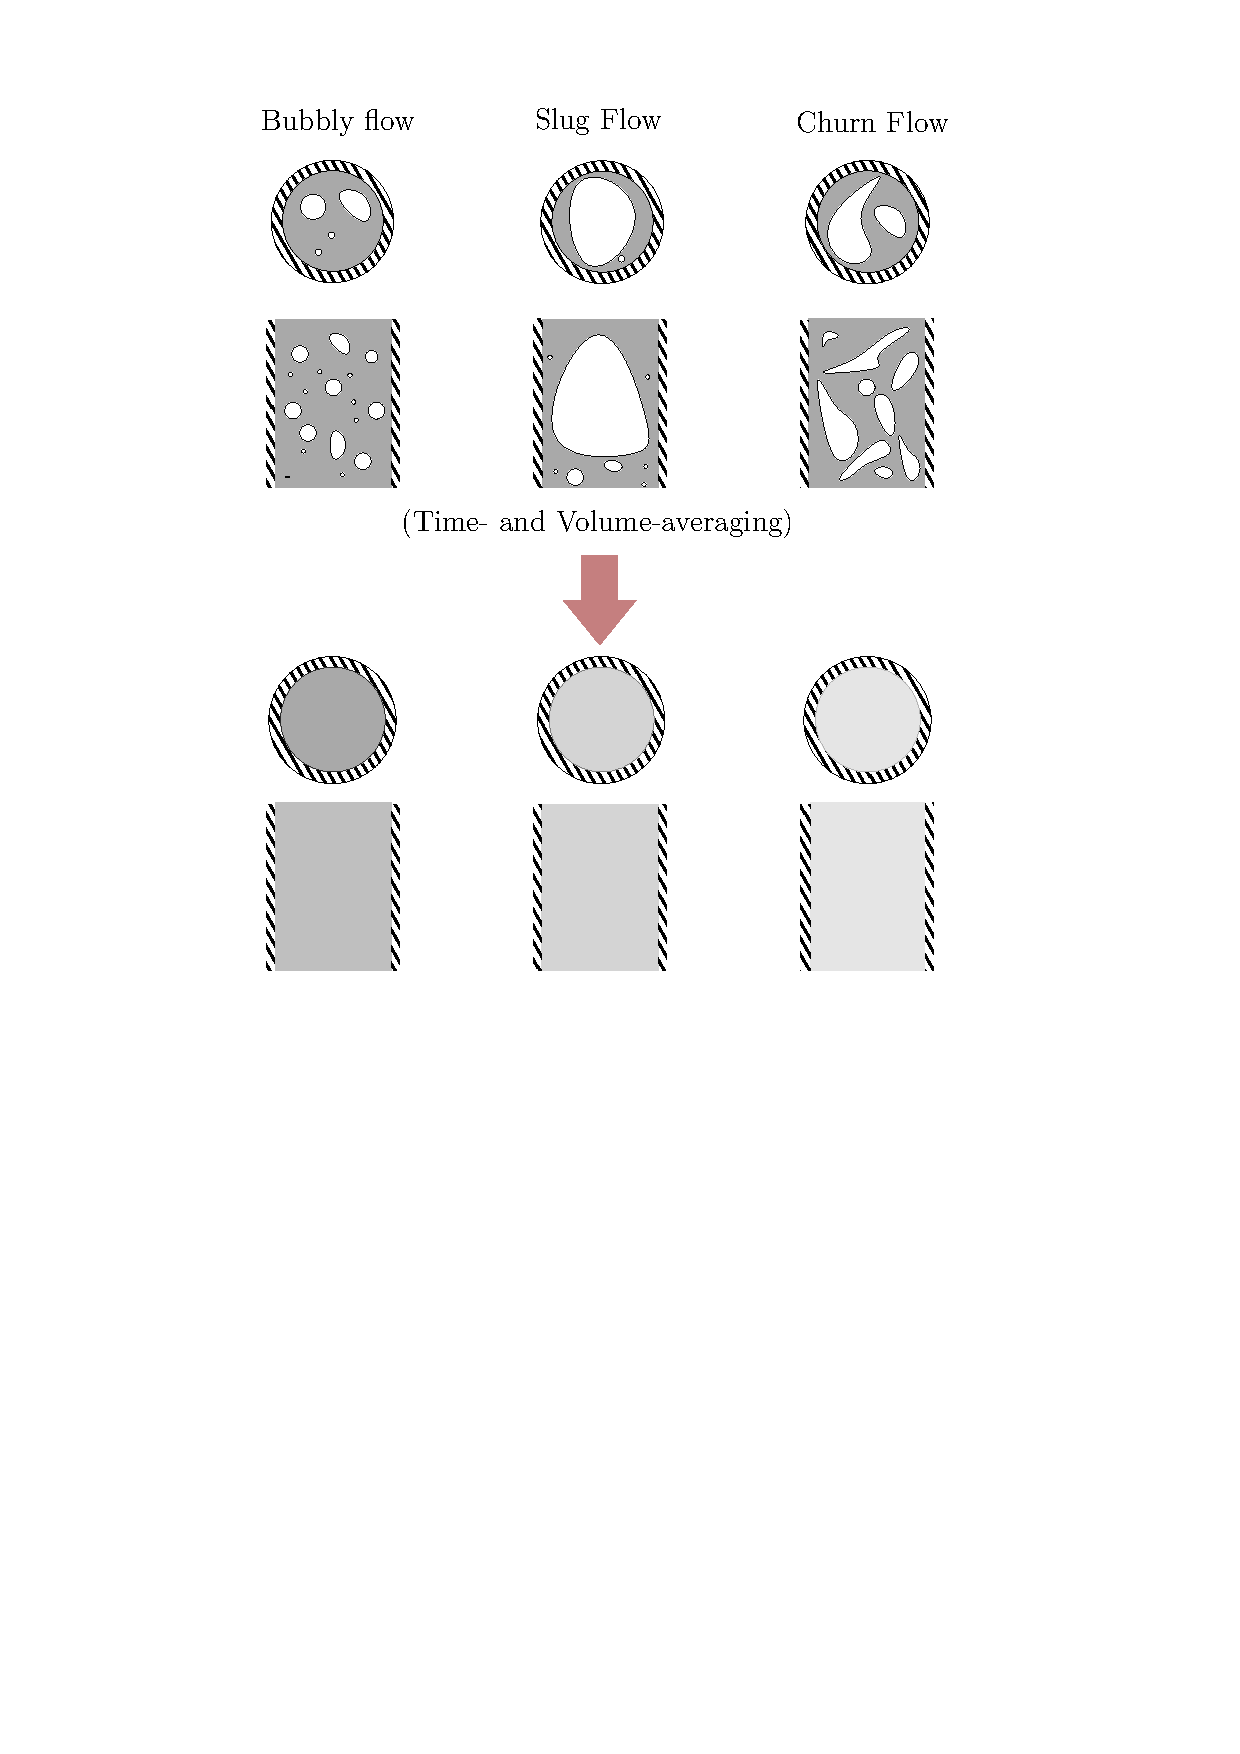
\includegraphics[scale=0.55]{../figures/chapter2/figures/flowAveraging}
	\caption[Illustration of Flow Averaging]{Time and volume average carried out on the two-phase flow inside a channel results in a tractable form of fluid dynamics equation, but incur loss of information at the local level, especially when it comes to the interfacial structure between phases and between each phase and the channel wall.}
	\label{fig:ch2_flow_averaging}
\end{figure}

% Opening Paragraph What is TRACE
\gls[hyper=false]{trace} is the best-estimate system \gls[hyper=false]{th} code developed by the \gls[hyper=false]{usnrc} as a tool for light water reactor transient analysis during normal and accident scenarios.
\marginpar{\gls[hyper=false]{trace} code}
Its development is an on-going effort to modernize into a single software package all previous \gls[hyper=false]{usnrc} \gls[hyper=false]{th} codes that were developed separately for specific reactor types and/or applications.
This ultimately would make the code more versatile for end users and more efficient to maintain for the developer.
Appendix~\ref{app:trace_consv_eqs} summarizes the final formulation of THE governing equations (time\- and volume-averaged) in \gls[hyper=false]{trace}, of which the complete derivation can be found in \cite{USNRC2012}.
In the next section the phenomenology of reflood is described and its modeling aspects with respect to the \gls[hyper=false]{trace} code are presented.
